\documentclass[a4paper, 12pt]{article}
\usepackage[utf8]{inputenc}
\DeclareUnicodeCharacter{00B2}{\ensuremath{{}^2}}
\usepackage{listings}
\usepackage{graphicx}
\title{Obligatorisk innlevering 1}
\author{Sivert M. Skarning}
\date{Mai 2019}
\begin{document}
\maketitle
\section{Oppgave 1}
\paragraph{Oppgavebeskrivelse}
Implementer konvolusjon på egen hånd. Implementasjonen skal være generell slik at den kan anvendes på alle bilder og filtere. Det er greit å begrense implementasjonen til å fungere på gråskalabilder, men det er ikke påkrevd. Implementasjonen skal støtte minst to ulike former for utvidelse/padding. Rapporten skal inneholde dokumentasjon for at implementasjonen fungerer.
\subsection{Dokumentasjon}
Vedlagt ligger et script kalt convolution.py. Koden utfører konvolusjon på bilde man legger ved som argument. Scriptet gir brukeren mulighet til å velge filterstørrelse of hvilke verdier filteret har. Brukeren har også mulighet til å velge mellom to forskjellige paddingmuligheter, zeropadding og reflectionpadding. Zeropadding er implementert med egenprogramert funksjon navngitt zero-pad.
Reflectionpad blir implmentert med pakken numpy og er navngitt np.pad. Begge funksjonene fungerer hvor zero-pad gir svart ramme rundt generert bild og reflectionpad gir utvidelse av bilde. Uten padding ville bruk av flere filtere etterhvert krympe bilde betydlig.
Selve implmentasjonen er inneffektivt implementert og i praksis ville man brukt en annen algoritme for å gjøre en konvolusjon. O-notasjonen for min implementsjon vil være: $$O(n² * m²)$$

\lstinputlisting[caption=Convolve function, language=Python, breaklines=true]{convolve.py}

\subsection{Resultat}
For å teste konvolveringsalgoritmen har jeg valgt å påføre tre typer filtere på lena.png.

\begin{figure}[h]
  \centering
  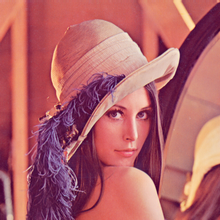
\includegraphics[width=0.5\textwidth]{images/lena}
  \caption{Bilde av Lena, et vanlig eksempel i bildebehandling}
  \label{fig:lena}
\end{figure}

\begin{itemize}
   \item Laplacian sharpening
   \item Mean blure
   \item Gaussian blure
\end{itemize}

\begin{figure}[h]
  \centering
  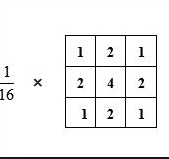
\includegraphics[width=0.5\textwidth]{images/gaussian-filter}
  \caption{Gaussian filter}
  \label{fig:gaussian-filter}
\end{figure}

\begin{figure}[h]
  \centering
  
\includegraphics[width=0.5\textwidth]{images/gaussian-blurred-lena}
  \caption{Lena konvolvert med filteret på Figur \ref{fig:gaussian-filter}}
  \label{fig:gaussian-blurred-lena}
\end{figure}

\paragraph{Gaussain blure} Konvolverings algoritmen fungerte bra. Her med egenimplementert zeropadding. Hadde først problemer med dårlig kontrast på bildet. Reskalerte intensiteten før bilde ble lagret, og fikk dermed et godt resultat som sett i figur \ref{fig:gaussian-blurred-lena}.

\paragraph{Mean blure}
Forskjellen mellom gaussian blure og mena blure for dette eksempelet er minimal. Ved større filtere ville man kunne se større forskjell. Man trenger vanligvis å kjøre gjennom et mean filter 4 ganger for å få den samme effekten som ved et gaussisk filter. Implementasjonen av konvolverings programmet er uheldig, da man heller skulle lagd det som et set med funksjoner man kunne kalle i steder for å lage det som et skript med bilde som argument. På denne måten kunne man ha testet større filtere lettere.

\begin{figure}[h]
  \centering
  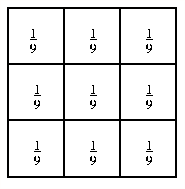
\includegraphics[width=0.5\textwidth]{images/mean-filter}
  \caption{Mean filter}
  \label{fig:mean-blure}
\end{figure}

\begin{figure}[h]
  \centering
  
\includegraphics[width=0.5\textwidth]{images/mean-blure-lena}
  \caption{Lena konvolvert med filteret på Figur \ref{fig:mean-blure}}
  \label{fig:mean-blurred-lena}
\end{figure}

\paragraph{Laplacian sharpening}
Laplacian filteret fremhever raske endringer i et bilde. På denne måten blir bilde skarpere, fordi vi kan se kantene på bilde bedere. Man vil se dette på figur \ref{fig:lena-laplacian} i forhold til figur \ref{fig:lena}.

\begin{figure}[h]
  \centering
  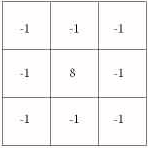
\includegraphics[width=0.5\textwidth]{images/laplacian-filter}
  \caption{Laplacian filter}
  \label{fig:laplacian-filter}
\end{figure}

\begin{figure}[h]
  \centering
  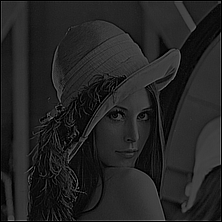
\includegraphics[width=0.5\textwidth]{images/laplacian-lena}
  \caption{Lena konvolvert med filteret på Figur \ref{fig:laplacian-filter}}
  \label{fig:lena-laplacian}
\end{figure}

\section{Opgave 2}
\paragraph{Oppgavebeskrivelse}
Implementer algoritmen for histogram spesifikasjon gitt i fagboka/slides. Implementasjonen må kunne brukes med ulike histogramspesikasjoner, så
dere må kunne lese inn et histogram. Det kan være greit å bruke et bilde til å representere et histogram. Sørg i tilfelle for at korrekt antall bøtter (piksler) og at de summerer til 255. Det er også mulig å bruke en tekstfil med f.eks. en rad til hver bøtte. Rapporten skal inneholde dokumentasjon for at implementasjonen fungerer.

\subsection{Dokumentasjon}
Histogram spesifikasjon er implementert. Bruker Cumulative distribution function til mapping.
Det som blir gjort i koden er å importere histogrammet fra et bilde inn i en fil for så å matche barbara.png histogrammet til histogrammet i filen.

Skriptet beregener histogrammet til begge bildene. Histogrammene viser forekomsten av intensitetsnivået til pikslene. Histogrammene blir så regnet om til å vise sannsynlighet for forekomsten av en gitt intensitetsverdi. Den kumulative sannsynlighetsfunksjone blir så beregnet ved å regne ved å legge til forrige sannsynlighetsverdi i rekken. Vi går så igjennom alle verdiene i histogrammet for orginalbildet. For hver verdi i orginalhistogrammet går vi gjennom alle verdiene i det spesifiserte histogrammet. Hvis verdien for den spesifiserte histogrammet er større eller lik verdien for det orginale histogrammet setter merkerer vi oss denne indexen og lagrer den i en annen array. Når man har gått gjennom alle verdiene. Vil vi sitte igjen med en mapping array som viser hvilken intensitet en intensitet i bilde må for at histogrammet skal matche. Programmet går så igjennom hele bilde og setter rikitig intensitetsverdi for hver piksel i bilde.

Gitt de kumulative distribusjonsfunksjonene til histogrammene $H_1(), H_2()$.
Vi finner så for hver intensitet $G_1$ hvilke $G_2$ som gjør at $F_1(G_1) = F_2(G_2)$. Ved å gjøre dette får vi mapping funksjonen forklart ovenfor\footnote{https://en.wikipedia.org/wiki/Histogram\_matching}.

\subsection{Resultat}
Skriptet fungerer fint og resultate stemmer med forventingen. Vi ser at figur \ref{fig:barbara-histogram} viser resultatet av histogram spesifikasjon med figur \ref{fig:barbara} som input og figur \ref{fig:specified-histogram} som spesifisert histogram. Vi ser at figur \ref{fig:barbara-histogram} er blir dominert av høyere intensitet. Dette er fordi figur \ref{fig:specified-histogram} også er dominert av høyere intensitet.

\begin{figure}[h]
  \centering
  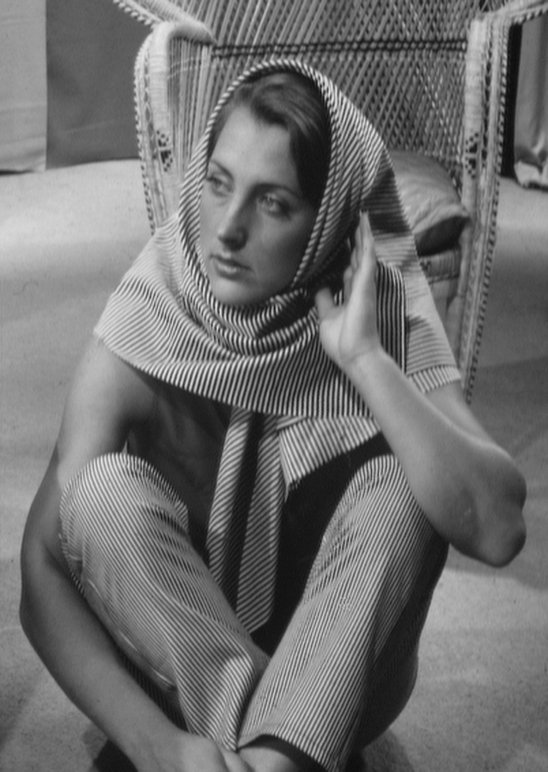
\includegraphics[width=0.5\textwidth]{images/barbara}
  \caption{Barbara}
  \label{fig:barbara}
\end{figure}

\begin{figure}[h]
  \centering
  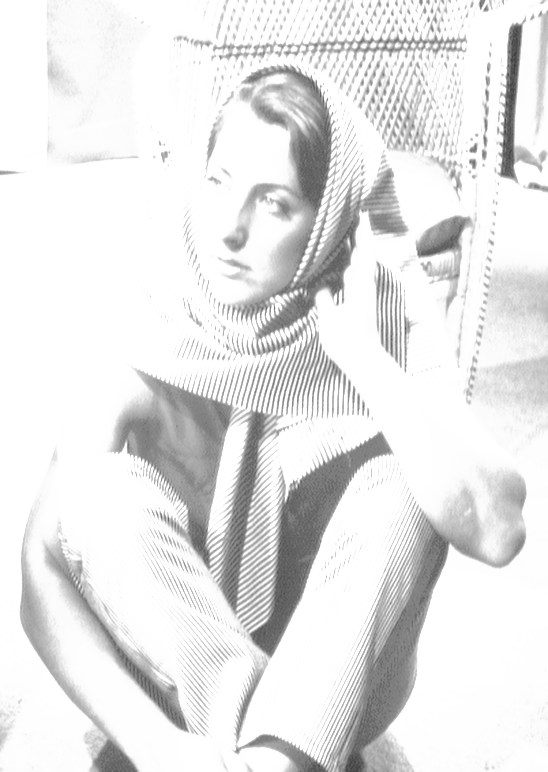
\includegraphics[width=0.5\textwidth]{images/barbara-histogram}
  \caption{Barbara etter histogram spesifikasjon}
  \label{fig:barbara-histogram}
\end{figure}

\begin{figure}[h]
  \centering
  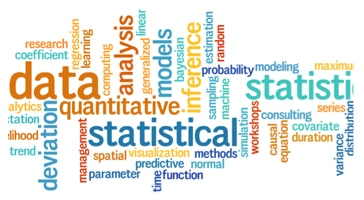
\includegraphics[width=0.5\textwidth]{images/specified-histogram}
  \caption{Det spesifiserte histrogrammet er tatt fra dette bilde}
  \label{fig:specified-histogram}
\end{figure}

\section{Oppgave 3}
\subsection{Oppgavebeskrivelse}
Utfør utjevning og skjærping på følgende bilder. Ulike metoder for både utjevning og skjærping skal utprøves og resultatet fra filtreringen skal dokumenteres i rapporten. Det er lov (anbefalt av ytelseshensyn) å ta i bruk innebygde innebygde implementasjoner for for å selve konvolusjonen.

\subsection{Implementasjon}
I denne oppgaven har jeg implementert funksjonalitet for fire spatiale filtere.
\begin{itemize}
\item Gaussian filter
\item Laplacian sharpening
\item Highboost filtering
\item Mean blure
\end{itemize}

\paragraph{Gaussian blure}
Gaussisk utjevning utjevner figur \ref{fig:barbara} bra. Et problem med gaussisk utjevning, som også blir observert her er at kantene på bilde ikke blir bevart spesielt bra.
På figur \ref{fig:barbara-noise-2} ser vi at bilde er preget av støy. Vi kan også se at gaussisk utjevning på figur \ref{fig:barbara-noise-2-5} at støyen er redusert. Også her ser vi at kantene på bilde ikke blir bra bevart.
\begin{figure}[h]
  \centering
  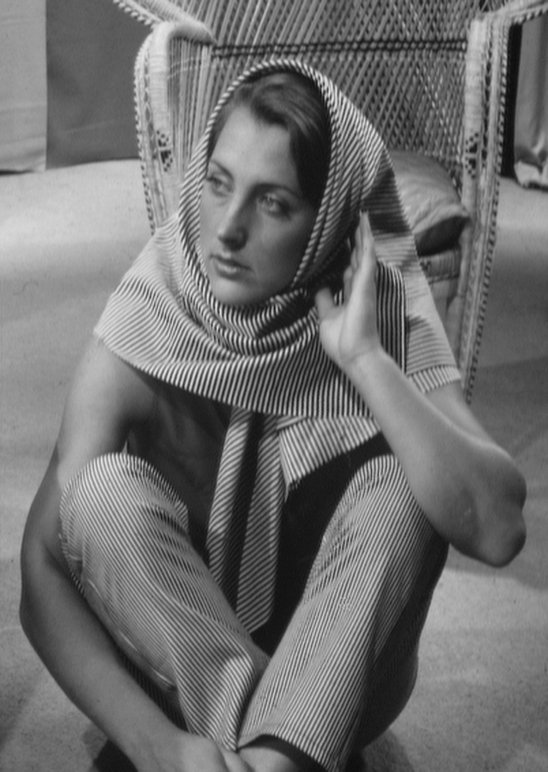
\includegraphics[width=0.5\textwidth]{images/barbara}
  \caption{Barbara}
  \label{fig:barbara}
\end{figure}

\begin{figure}[h]
  \centering
  
\includegraphics[width=0.5\textwidth]{images/barbara-gaussian-5}
  \caption{Barbara gaussian, standardavvik: 5}
  \label{fig:barbara-gaussian-5}
\end{figure}

\begin{figure}[h]
  \centering
  
\includegraphics[width=0.5\textwidth]{images/barbara-gaussian-20}
  \caption{Barbara gaussian, standaravvik 20}
  \label{fig:barbara-gaussian-20}
\end{figure}

\begin{figure}[h]
  \centering
  
\includegraphics[width=0.5\textwidth]{images/barbara-noise-1}
  \caption{Barbara med støy}
  \label{fig:barbara-noise-1}
\end{figure}

\begin{figure}[h]
  \centering
  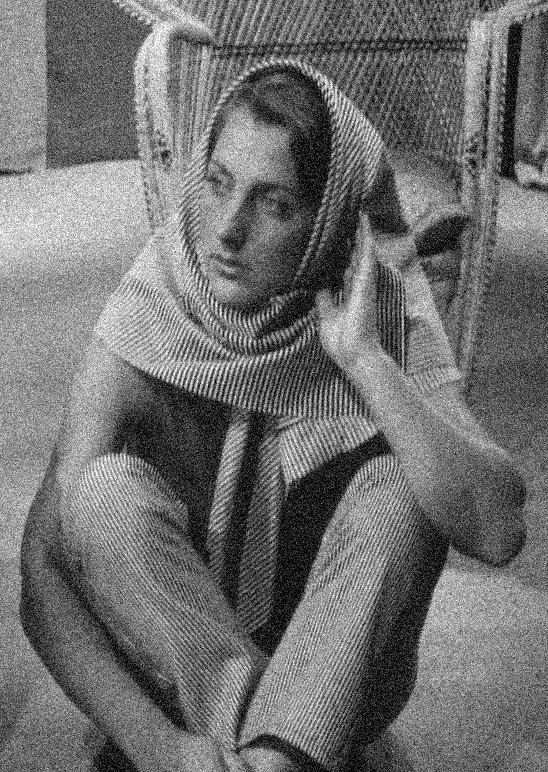
\includegraphics[width=0.5\textwidth]{images/barbara-noise-2}
  \caption{Barbara med mer støy}
  \label{fig:barbara-noise-2}
\end{figure}

\begin{figure}[h]
  \centering
  
\includegraphics[width=0.5\textwidth]{images/gaussian-noise-1-5}
  \caption{Barbara med støy, utjevnet med standardavvik på 5}
  \label{fig:barbara-noise-1-5}
\end{figure}

\begin{figure}[h]
  \centering
  
\includegraphics[width=0.5\textwidth]{images/barbara-noise-2-5}
  \caption{Barbara med mer støy, utjevnet med standardavvik på 5}
  \label{fig:barbara-noise-2-5}
\end{figure}

\paragraph{Mean blure}
Mean blure er en veldig grunnleggende utjevningsmetode. Den er raskere en det gaussisk utjevning er, og den bevarer kantene bedre. Den er dog ikke like effektiv til å fjerne støy.
Mean blure med et 5x5 filter med pixel verdier på $1/25$ kan bli sett i figur \ref{fig:barbara-mean-blure}

\begin{figure}[h]
  \centering
  
\includegraphics[width=0.5\textwidth]{images/barbara-mean-blure}
  \caption{Mean blure}
  \label{fig:barbara-mean-blure}
\end{figure}

\paragraph{Laplacian sharpening}
En Lapllacian operator er et godt valg for å fremheve detaljer i bilde. Dette vil si at kantene blir fremhevet. På figur \ref{fig:laplacian-sharpening} ser vi at bilde har veldig lav kontrast. Usikker på hva som forårsaker dette resultatet. De kantene som er synlige er fremhevet so forventet.

\begin{figure}[h]
  \centering
  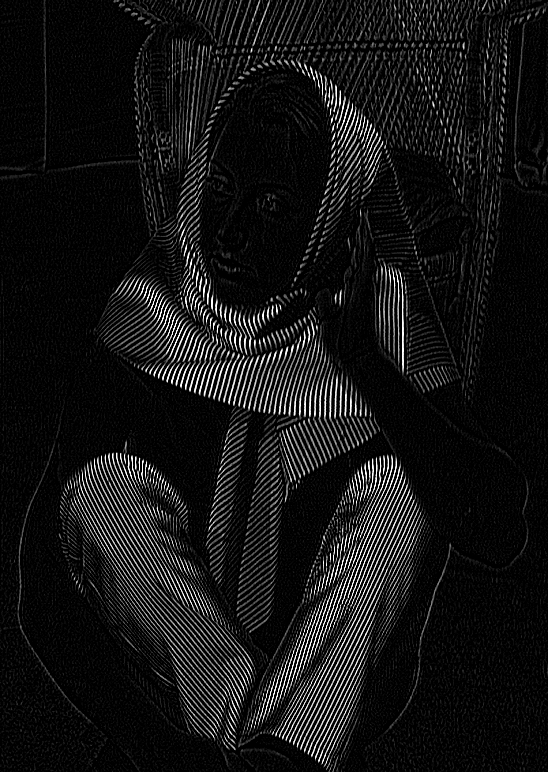
\includegraphics[width=0.5\textwidth]{images/laplacian-sharpening}
  \caption{Laplacian sharpening}
  \label{fig:laplacian-sharpening}
\end{figure}

\paragraph{Higboost filtering}
Highboost filtering er en teknikk hvor man forsterker kantene og fjerner delen av bilde som ikke er skarpt. I figur \ref{fig:highboost-filtering}, ser vi at kantene er fremhevet. Deler av koden i denne implementsjonen er tatt fra \footnote{https://github.com/lavima/itd33517\_examples/blob/master/lecture05\_highboost.py}. Higboost filtering fungerer ved at man trekker i fra et utjevnet versjon av bilde. Dette fører til at man beholder både de lav og de høye frekvensene i bilde samtidig som kantene blir fremhevet \footnote{https://www.scribd.com/doc/119044470/High-Boost-Filtering} 

\begin{figure}[h]
  \centering
  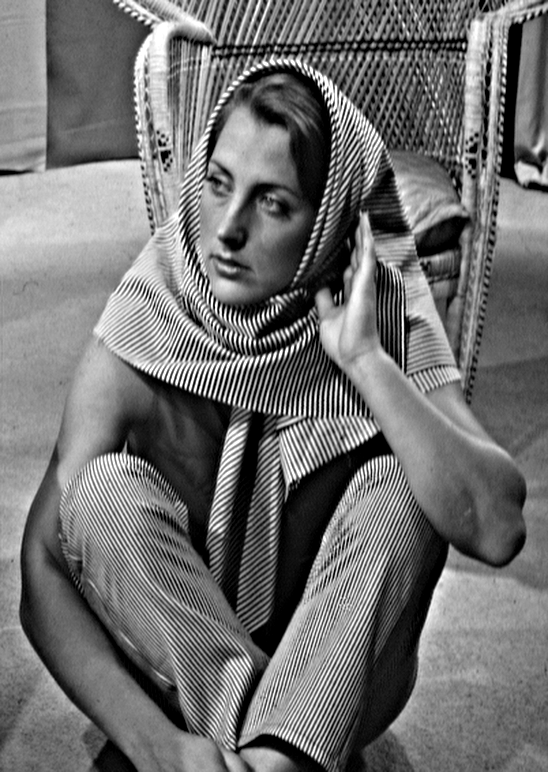
\includegraphics[width=0.5\textwidth]{images/highboost-filtering}
  \caption{Barbara highboost filtering}
  \label{fig:highboost-filtering}
\end{figure}

\end{document}


